% Drawing 136/18-1 -- folder 136, batch 18, archive page 356 (PDF page 357).
% Transcription: sous deux crochets illisibles, un faisceau de segments reliant deux colonnes de points : l’image d’un shuffle.
% Kind: shuffle: segments between two columns of points. Method 2 (schematic redraw from the facsimile). Status: ok.
% Notes: Redrawn on a tight crop. Nine strokes between a left column of five marks and a right column of five marks (drawn as points): the four upper ones descend steeply to the right and cross, the next three are nearly horizontal and end on the first three right points, the two lowest are slightly curved (the last runs past the right column). The two bracketed labels above are struck/illegible and left out. Still a reading: which strokes start at which left mark (most start just beside the column, not on a mark), and the marks themselves (small ticks, two heavy points). Redrawn 2026-11-09 (issue 128): to check again. 2026-11-13, Claude Opus 5.5, overlay check (issue 147): not compiled (no TeX in the session); the TikZ rasterised and laid over the 259 ppi colour scan (rendered at 350 dpi). Redrawn: the nine strokes were straight lines up to 2 units off their ink; each is now drawn through points read on it, and lies on the ink to within about 0.5 unit. Read on the page: the four upper strokes start beside the left column (at about y = 30.5, 38, 45, 51) and end at about (79.5, 59.4), (68.7, 61.4), (62.1, 58.7), (57.9, 61.1); the fourth (blue) crosses the fifth near x = 30; the fifth runs from the second left mark to the first right point; the sixth and seventh end at the hook and at the slash of the right column; the eighth curls down just before the blue blot; the ninth runs past the column and curls up at its end. The marks are drawn as they are instead of as uniform points: on the left a tick at 44, a tick at 55, a heavy vertical blot at 61, a heavy point with a hooked tail at 69, a tick and a short oblique stroke at 81-85; on the right a heavy point with a short tail at 54, a hook ending in a dot at 64-66, a short slash at 73-74.5, a heavy point at 76 and a filled blot at 85. Left out: the two bracketed words above, which are blotted out (crossings-out, not part of the figure), and three faint specks of the left column (at 33, 47 and 89).
% Coordinates: 1 unit = 1 mm = 1/100 of the crop width (bbox in page fractions: [0.75, 0.27, 0.88, 0.36]).
% Redrawn by Claude (claude-opus-5-5), issue #73, 2026-11-09; not checked by a human; not compiled (no TeX in the session).
% Revised by Claude Opus 5.5 (claude-opus-5-5), issue #147, 2026-11-13: overlay check on the colour scan; not checked by a human; not compiled (no TeX in the session).
% Rights: reproduces part of the work -- behind RENDER_TRANSCRIPTS, never published by itself.
\documentclass[tikz,border=3pt]{standalone}
\usepackage{amsmath,amssymb}
\usetikzlibrary{patterns,arrows.meta}
\tikzset{pencil/.style={black!45}, struck/.style={black!35}, mark/.style={circle,draw,inner sep=1.3pt}, pt/.style={circle,fill,inner sep=0.9pt}, opt/.style={circle,draw,fill=white,inner sep=1.1pt}}
\begin{document}
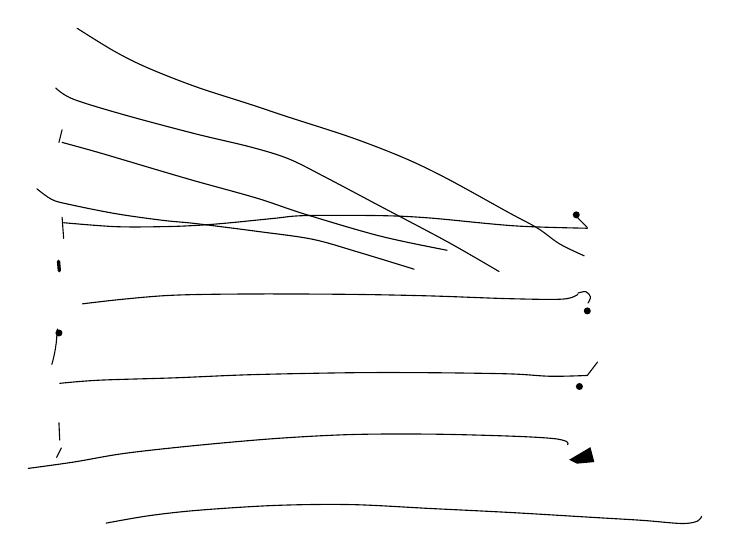
\begin{tikzpicture}[x=1mm,y=1mm,line cap=round,line join=round,font=\scriptsize]
\draw plot[smooth, tension=0.55] coordinates {(15.1,-30.5) (19.8,-33.4) (24,-35.5) (30.1,-37.9) (37.2,-40.2) (42,-41.8) (50,-44.4) (56.7,-47) (62.1,-49.6) (69.9,-53.9) (73.6,-55.9) (76.4,-57.9) (79.5,-59.4)};
\draw plot[smooth, tension=0.55] coordinates {(12.4,-38.1) (14.6,-39.5) (21.1,-41.5) (30.1,-43.9) (37.2,-45.6) (42,-47.1) (46.8,-49.5) (53.6,-53.1) (62.1,-57.6) (68.7,-61.4)};
\draw plot[smooth, tension=0.55] coordinates {(13.2,-45) (17.9,-46.3) (24.3,-48.2) (30.1,-49.9) (38,-52.1) (44,-54.1) (53.6,-56.9) (62.1,-58.7)};
\draw plot[smooth, tension=0.55] coordinates {(10,-50.9) (11.9,-52.25) (14,-52.85) (20,-54.05) (26,-54.9) (30.1,-55.3) (38,-56.3) (45,-57.3) (50.7,-58.9) (57.9,-61.1)};
\draw plot[smooth, tension=0.55] coordinates {(13.4,-55.2) (20,-55.7) (26,-55.7) (30.1,-55.55) (34.1,-55.25) (40.1,-54.65) (44,-54.3) (53.6,-54.3) (59.9,-54.6) (70.7,-55.6) (79.9,-55.9)};
\draw plot[smooth, tension=0.55] coordinates {(15.8,-65.5) (21.1,-64.9) (27.5,-64.4) (37.2,-64.25) (50,-64.3) (60.1,-64.5) (70.1,-64.85) (76.8,-64.9) (78.7,-64.3)};
\draw plot[smooth, tension=0.55] coordinates {(12.9,-75.6) (17.9,-75.2) (27.5,-74.9) (37.2,-74.5) (50,-74.25) (60.1,-74.25) (70.1,-74.4) (75.2,-74.7) (79.9,-74.6)};
\draw (79.9,-74.6) -- (81.2,-72.9);
\draw plot[smooth, tension=0.55] coordinates {(8.9,-86.4) (14.65,-85.6) (21.1,-84.5) (30.1,-83.5) (40.4,-82.6) (50,-82.1) (60.1,-82.05) (70.1,-82.3) (75.5,-82.6) (77.3,-83) (77.4,-83.4)};
\draw plot[smooth, tension=0.55] coordinates {(18.8,-93.35) (24.3,-92.4) (30.7,-91.7) (40.4,-91.1) (50,-91) (60.1,-91.5) (70.1,-92) (80.2,-92.6) (86.9,-93) (91.9,-93.4) (93.9,-93.1) (94.4,-92.5)};
\draw (13.2,-43.4) -- (12.8,-45);
\draw (13.2,-54.5) -- (13.4,-57.2);
\draw[very thick] (12.75,-60.1) -- (12.85,-61.3);
\node[pt] at (12.8,-69.2) {};
\draw plot[smooth, tension=0.55] coordinates {(12.6,-68.7) (12.45,-70.5) (12.2,-72) (11.9,-73.2)};
\draw (12.8,-80.6) -- (12.9,-82.8);
\draw (13.1,-83.8) -- (12.5,-85);
\node[pt] at (78.5,-54.2) {};
\draw (78.7,-54.6) -- (79.9,-55.8);
\draw plot[smooth, tension=0.55] coordinates {(78.7,-64.15) (79.7,-63.95) (80.3,-64.6) (80,-65.4)};
\node[pt] at (79.9,-66.4) {};
\node[pt] at (78.9,-76) {};
\fill (77.6,-85.3) -- (80.3,-83.7) -- (80.8,-85.6) -- (78.6,-85.8) -- cycle;
\end{tikzpicture}
\end{document}
